\chapter{Mains}

\ChapterIntro{
    \lettrine{T}{his is the} chapter intro. \lipsum[1-3]
}

%
%
% Mr. Kim's Seattle-style Spicy Teriyaki
%
%
\newpage

\RecipeNameAndYield{Name=Mr. Kim's Seattle-style Spicy Teriyaki}

\RecipeStory{\lettrine{W}{e moved to Southern California} at the beginning of 2021 and the one thing
    that we really missed was Mr. Kim's spicy chicken teriyaki. Caitlyn would
    ask for it all the time, but there was nothing we could do. Seattle-style
    teriyaki is very different from traditional Japanese teriyaki. Very different.

    We like to serve this will extra sauce over white rice. Add more sambal to taste.}

\begin{IngredientsAndSteps}
    \ListIngredientsAndSteps
    {
        1 cup tamari

        1 cup white sugar

        1\fr1/2 \tsp[s] light brown sugar

        10 cloves garlic, smashed and minced

        3 \Tbl[s] grated fresh ginger

        \fr1/4 \tsp black pepper

        1 \tsp cinnamon

        1 \Tbl pineapple juice

        3 \Pd[s] skinless boneless chicken thighs

        2 \Tbl[s] cornstarch

        8 \Tbl[s] sambal oelek
    }
    {
        In a small saucepan, combine all ingredients except chicken, cornstarch, and sambal.
        Bring to a boil over high heat. Reduce heat to low and stir until all the sugar is
        dissolved. Remove from heat and let cool a bit. Mix in \fr1/2 cup of water.

        Clean and trim chicken thighs and divide into two heavy duty ziplock bags. Divide the
        sauce and put half in each bag. Press the air out and seal the bags. Let marinate 30 - 60
        minutes (or longer).

        Remove chicken and set aside. Put the marinade into a small saucepan and bring back
        to a boil. Reduce heat to low. Combine cornstarn and 2 \Tbl[s] of cold water and
        add to the pan while constantly stirring. Cook down until slightly thickened. You might
        want to add up to \fr1/2 cup of water to keep a consistent thickness. (Yeah, we know, this
        is conflicting information...)

        Preheat the grill to very hot. Spray grill with nonstick cooking spray and reduce
        heat to medium. Grill chicken until done (about 8 minutes per side). Next, increase grill
        heat to very hot so that you get a good crispness and char on the chicken.

        Slice or dice the chicken and put in a bowl. Combine the sambal and teriyaki sauce in
        a small bowl and pour over the chicken.
    }

\end{IngredientsAndSteps}

%
%
% Dads's Meatballs
%
%
\newpage

\RecipeNameAndYield{Name=Dads's Meatballs, Yield=Makes about 40 meatballs}

\RecipeStory{\lettrine{T}{stuff goes here} \lipsum[2]}

\begin{IngredientsAndSteps}
    \ListIngredientsAndSteps[Meatballs]
    {
        3 16 \Ounce packages of ground turkey

        2 16 \Ounce packages of Italian turkey sausages

        2 16 \Ounce packages of turkey breakfast sausage

        1 bunch Italian parsley (about 1 cup)

        1 bunch basil (about 4 \Tbl[s] chopped)

        3 cups Italian white bread, crust removed and diced

        1 cup whole milk

        3 eggs

        1 medium shallot

        \fr1/2 head of garlic (about 8 to 10 cloves)

        2 \Tbl[s] red pepper flakes

        2 teapoons salt

        2 teapoons pepper
    }
    {
        Start by soaking the diced bread in the cup of milk for at least 10 minutes. You want the bread to be
        soft and nearly falling apart. While the bread is soaking coursely chop the shallots, garlic, basil,
        and parsley, and put them into a food processor.  Add the garlic and shallots to the food processor.
        When the bread is ready, squeeze a bit of the milk out, add \fr1/2 of it and \fr1/2 \Pd
        of the ground turkey to the food processor and process until most of ``those green thingies'' are
        ground up and no longer really visible. Remove the turkey from the food processor to a large bowl, add the
        remaining bread and another \fr1/2 \Pd of ground turkey.

        Peel the Italian sausages by slicing them lengthwise and removing the casing. Put the peeled sausages,
        breakfast sausage, remaining turkey, salt, pepper, and two eggs into a very large bowl. Scrap the turkey
        from the food processor into the bowl. Now, smoosh it all together until everything is evenly mixed.

        Spray two large jelly roll pans with PAM. Measure 3\fr1/2 \Ounce portions of the meat and form them
        into firm balls. Place these on the jelly roll pans. You'll end up filling both of the pans. When you're done
        making the meatballs put them in a 425 degree oven until they are cooked on the outside and read around
        165\Degrees[F] with an instant-read thermometer.
    }

    \ListIngredientsAndSteps[Sauce]
    {
        2 32 \Ounce cans of crushed tomatoes

        1 32 \Ounce can of tomato sauce

        1 32 \Ounce can of diced tomatoes

        3 \Tbl[s] olive oil

        3 medium shallots, diced

        \fr1/2 head of garlic (about 8 to 10 cloves)

        1 bunch basil, (about 4 \Tbl[s] chopped)

        2 \Tbl[s] red pepper flakes

        1 \Tbl salt

        1 \Tbl pepper
    }
    {
        While the meatballs are baking heat the olive oil over a medium flame in a very large heavy bottomed Dutch oven.
        I prefer the the 4 gallon All Clad for this. Add the shallot and garlic and cook until fragrant and the shallots
        and garlic are translucent. Add the tomatoes starting with the diced ones (to reduce splashing). Add the remaining
        ingredients. Fill one of the 32 \Ounce tomato cans with warm water and add to the pot.
    }

    \ListIngredientsAndSteps[Putting it all together]
    {}
    {
        When the meatballs are done add them to the pot one at a time. Turn the sauce down to low-medium and let simmer
        for 2 or 3 hours. Make sure to stir about every 15 minutes to keep the sauce from burning and to make sure all the
        meatballs get a chance to cook under the sauce. You might need to keep adding water if the sauce starts to get too
        thick.
    }

\end{IngredientsAndSteps}

%
%
% Caitlyn's Fried Chicken Fingers
%
%
\newpage

\RecipeNameAndYield{Name=Caitlyn's Fried Chicken Fingers}

% \begin{figure}
%     \centering
%     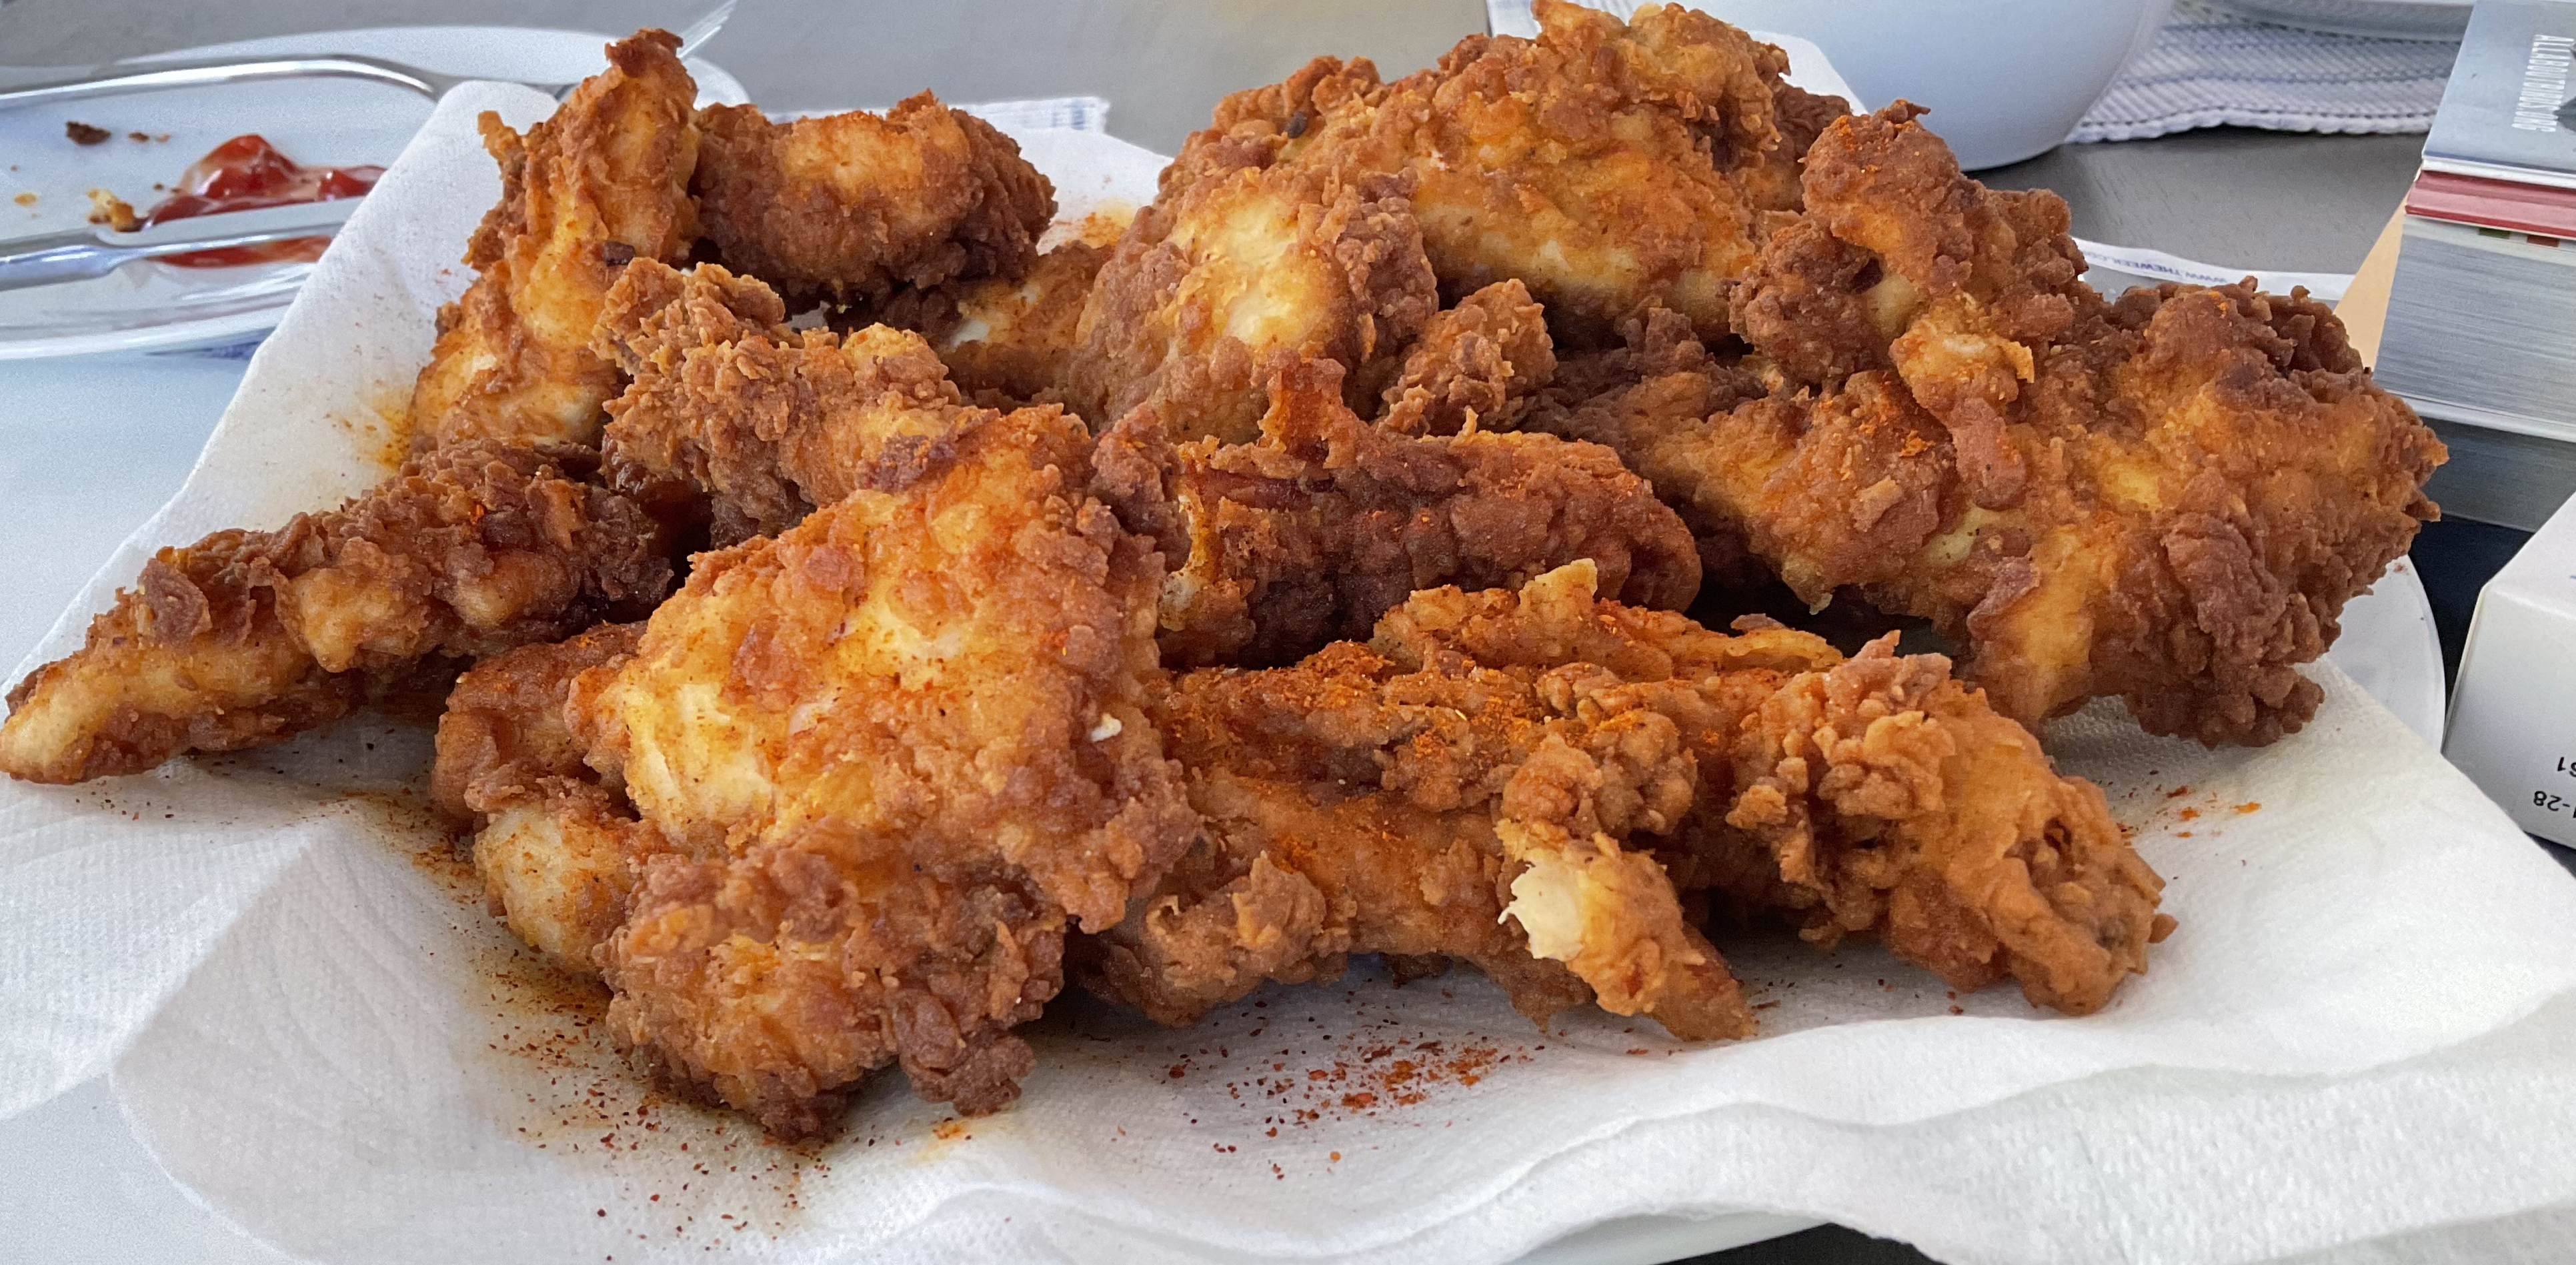
\includegraphics[scale=0.095]{../images/fried-chicken.png}
% \end{figure}

\RecipeStory{\lettrine{S}{ometimes you just need to start} with someone's recipe and then tweak the hell out of it until it works.
    This is one of those times. This started as a TikTok recipe, but, well, it was a little rough. Not all
    the ingredients were listed. Actually, let's face it, \emph{nothing} was really written down. There were
    two places where ``1 \Tbl All-purpose'' was listed. ``All-purpose \emph{what}'', exactly? Anyway, Caitlyn wanted to make these
    and took a real run at them. After the first three pieces came out
    less than perfect (in Caitlyn's words), she made some changes, and this is the result.}

\begin{IngredientsAndSteps}
    \ListIngredientsAndSteps[Dry part]
    {
        4 cups flour

        2 \Tbl[s] baking powder

        2 \Tbl[s] garlic powder

        2 \Tbl[s] onion powder

        1 \Tbl cayenne pepper

        1 \tsp black pepper

        1 \tsp salt

        cayenne, chili powder, ancho chili, or other flavorful spice for sprinkling, to taste
    }
    {}

    \ListIngredientsAndSteps[Wet part]
    {
        1\fr1/4 cup cultured buttermilk

        \fr1/4 cup pickle juice

        1 \Tbl miced garlic

        \fr1/2 \Tbl garlic powder

        \fr1/2 \Tbl onion powder

        1 \Tbl cayenne pepper

        1 \Tbl black pepper

        1 \Tbl baking soda

        1\fr1/2 \Pd[s] (one package) chicken tenders
    }
    {}

    \ListIngredientsAndSteps[Then...]
    {
    }
    {
        Cut chicken into smallish pieces (about 2 \Ounce[s] each) and pound flat in a double zipper lock bag. You can
        use your hands or a mallet. Just don't make them too thin. Nobody likes a thin chicken finger. Set this aside.

        Combine all the dry ingredients in a medium-sized bowl. Combine all the wet ingredients in a medium-sized bowl. In a few
        minutes this should start to bubble on its own. This
        is a good thing because it makes the batter nice and light.

        Bring a heavy bottom dutch oven with about 2 inches of canola, corn, or other vegetable oil to somewhere between
        365 and 375\Degrees[F]. It's important that the oil remain in this range. Too hot and you'll burn the outside of the
        chicken, but leave the inside raw. Too low and it'll take forever to cook while soaking up all the oil. Neither
        are a win. Later, when frying the chicken, keep an eye on this temperature and adjust as necessary.

        When the oil is ready drop a few pieces of the chicken into the buttermilk batter and make sure they get fully
        covered. Pick them up one at a time and let the buttermilk drip off a bit. Dip each piece of battered chicken into
        the dry ingredients and make sure it gets flour all the way around. Place the battered chicken on a tray.

        When you have 4 or 5 pieces ready it's time to drop them into the hot oil. Shake off any excess flour before putting
        the tenders in the oil. Cook about 4 minutes on one side, turn over with a long-handled tong, then cook until they are
        at least 165\Degrees[F] inside. Place them on a paper towel and sprinkle with the cayenne and chili powder. The more, the
        spicier. And spicier is good.
    }
\end{IngredientsAndSteps}

%
%
% Chicken Lettuce Wraps
%
%
\newpage

\RecipeNameAndYield{Name=Chicken Lettuce Wraps}

\RecipeStory{\lettrine{T}{his recipe is an adaptation} of the PF Chang's Chicken Lettuce Wraps
    recipe found on Damn Delicious. We make a pot of white rice and serve
    this with butter or iceberg lettuce. It's important to use ``regular''
    soy sauce for this recipe. We've found that using low sodium tends
    to leave the overall flavor a little too sweet.}

\begin{IngredientsAndSteps}
    \ListIngredientsAndSteps
    {
        1 \Tbl olive olive

        1 \Pd ground chicken

        3 cloves garlic, smashed

        \fr1/4 cup hoisin sauce

        2 \Tbl[s] soy sauce (don't use low-sodium)

        1 \Tbl rice wine vinegar

        1\fr1/2 \Tbl[s] sambal oelek

        2 \Tbl[s] grated fresh ginger

        1 small yellow onion, diced very small

        2 green onions, sliced thin

        (optional) 1 (8-\Ounce) can water chestnuts, drained and diced

        kosher salt and pepper to taste (about \fr1/2 \tsp each)
    }
    {
        Combine garlic, hoisin, soy, vinegar, and sambal, then side aside.

        Heat olive oil in deep skillet over medium high heat. Reduce heat to medium, add ground chicken,
        and cook until browned, about 10 minutes, making sure to crumble the chicken as it cooks.

        Add yellow onion, grated ginger, and sauce combination to chicken and allow to cook until
        onions are translucent.

        Stir in green onions and cook until tender, about 2 minutes; season with salt
        and pepper, to taste. If using water chestnuts add them at this time and cook
        until they are warmed through.
    }
\end{IngredientsAndSteps}

%
%
% Mom's Meatballs
%
%
\newpage

\RecipeNameAndYield{Name=Mom's Meatballs}

\RecipeStory{\lettrine{T}{his sorta, kinda, started} as Nana's meatballs recipe and she would make it
    every time Caitlyn when to their house in Redmond. Well, Mom took that recipe, made a few changes
    and made it her own. Of the two Miller meatball recipes, this is Caitlyn's favorite.}

\begin{IngredientsAndSteps}
    \ListIngredientsAndSteps[Meatballs]
    {
        2 16 \Ounce packages of ground turkey (93\% Lean)

        1 piece of bread

        1 egg

        1 large clove of crushed garlic

        1\fr1/2 tsp of oregano
    }
    {}

    \InsertHiddenLines{3}

    \ListIngredientsAndSteps[Sauce]
    {
        3 cans of 32\Ounce crushed tomatoes

        1 medium shallot (chopped fine)

        3 cloves of garlic (sliced thin)

        3 \Tbl[s] of olive oil

        1 tsp of basil

        1 tsp of oregano

        1 tsp of parsley

        Salt, pepper, and red pepper flakes to taste
    }
    {
        To prepare the sauce, sauté the onions and garlic in olive oil until translucent. Be careful because you don't want to burn
        them.

        Add the 3 cans of crushed tomatoes, basil, oregano, and parsley and stir until combined.

        Let this simmer for about 30 minutes.
    }

    \InsertHiddenLines{3}

    \ListIngredientsAndSteps[Putting it all together]
    {}
    {
        Add the meatballs to the sauce one a time and cook for at least 1\fr1/2 hours. Stir every 15 minutes or so to make
        sure that the sauce doesn't burn and that the meatballs get well cooked.

        You can check the meatballs are done using an instant read thermometer inserted into the middle of a meatball.
        They are ``done'' when the temperature reaches 165\Degrees[F]. It's ok to cook them longer.
    }
\end{IngredientsAndSteps}

%
%
% Tuna pasta salad
%
%
\newpage

\RecipeNameAndYield{Name=Tuna pasta salad}

\RecipeStory{\lettrine{T}{stuff goes here} \lipsum[2]}

\begin{IngredientsAndSteps}
    \ListIngredientsAndSteps
    {
        2 cans white albacore tuna

        1 cup chopped dill pickles

        \fr1/2 \tsp salt

        1 teapoon Lawry's seasoning

        \fr1/4 teapoon dried basil

        \fr1/4 teapoon black pepper

        1 cup cottage cheese

        \fr1/2 cup sour cream

        \fr1/4 cup mayonnaise

        2 teapoons yellow mustard

        1 box medium shells, penne, or other fun shapes
    }
    {
        Boil the pasta until it's just slightly over-cooked. Drain, rinse, and cool.

        Mix the salt, Lawry's, basil, pepper, cottage cheese, sour cream, mayonnaise, and mustard in
        a large bowl.

        Put the cooled pasta into the wet ingredients and mix well.

        Add the remaining ingredients and combine.

        Now, this is up to you, but most people might put this in the fridge for a few hours to chill,
        but not Caitlyn. She prefers it slightly warm and much more wet.
    }
\end{IngredientsAndSteps}

